\documentclass[12pt,parskip=half-, twoside=semi]{scrartcl}
\usepackage[T1]{fontenc} % encodage des caractères
\usepackage[french]{babel} % texte en français
\usepackage{microtype} % meilleur justification du texte
\usepackage{cmbright} % police sans serif
\usepackage[frenchmath]{mathastext} % pour le lettres majuscules droites
\usepackage{stmaryrd} % \sslash pour le symbole parallèle
\usepackage{mathtools}
\usepackage{graphicx}
\usepackage{tikz, tkz-euclide}
\usepackage{gensymb}
\usepackage{enumitem}
\setlist[enumerate]{label=\alph*)}
\usepackage{tcolorbox}
\usepackage{gensymb}
\usepackage{multicol}
\NewDocumentCommand{\dotsforanswer}{m o O{1ex}}%
{%
    \IfNoValueTF{#2}%
    {
        \foreach \i in {1,...,#1}{\dotfill\vskip #3}
    }
    {
        #2\dotfill\vskip #3
        \foreach \i in {2,...,#1}{\dotfill\vskip #3}
    }

}
\SetEnumitemKey{cols}
{
    itemsep= 1em,
    before = \raggedcolumns\begin{multicols}{#1},
    after = \end{multicols},
}
\usepackage{tcolorbox}
\newtcbox{\blackbox}{%
    on line,
    left=0pt,
    right=0pt,
    bottom=0pt,
    top=0pt,
    sharp corners,
    colframe=black,
    colback=black,
    coltext=white,
    fontupper=\bfseries
}


%%%%%%%%
% XSIM %
%%%%%%%%
\usepackage[use-files, use-aux]{xsim}
% Pour le template de l'interrogation
\DeclareExerciseEnvironmentTemplate{interrogation_template}%
{%
    \GetExercisePropertyTF{points}%
    % s'il y a des points
    {
        \blackbox%
        {%
            \XSIMmixedcase{\GetExerciseName}~\GetExerciseProperty{counter}%
        }%
        \hfill
        \blackbox{
            \GetExerciseProperty{points}
        }
        \par
    }
    % sinon
    {
        \blackbox%
        {%
            \XSIMmixedcase{\GetExerciseName}~\GetExerciseProperty{counter}%
        }%
        \par
    }%
}%
{%
    \par%
}
\xsimsetup{
    exercise/template = interrogation_template,
    solution/template = interrogation_template,
    exercise/name = question,
}

% Changer le titre ici
\newcommand{\montitre}{Devoir - Mai 2023}
% Changer la date ici
%\newcommand{\madate}{Lundi jj mm aaaa}


% En-tête et pied de page
\usepackage{scrlayer-scrpage}
\setlength{\headheight}{50pt}
\lohead{Nom :\\Prénom :\\Classe :}
\rohead{\no~\fbox{\phantom{XX}}\\~\\ Date : }

\begin{document}
% Titre
\begin{huge}
    \bfseries
    \montitre
    \hfill
    \dots/\TotalExerciseGoal{points}{}{}
    \bigbreak
\end{huge}

\emph{Sur feuille à entête}

\begin{exercise}[points=8]
	Effectue. 
	\begin{enumerate}[cols=2, itemsep=.2cm]
		\item \(4+5\cdot (-7)-13\)
		\item \(\left(-3+10\right)\cdot 2^3\)
		\item \(\left(8+(-3)\right)^2 - 120\)
		\item \(-4+(-2)-(-7)\)
		\item \(1^9 + 3^3 - 30 + 13\)
		\item \(-10+(-5) + \left(7-13\right)\)
		\item \(45:9\cdot 3 \)
		\item \(-9-13+2\cdot (-5+7)\)
	\end{enumerate}	
\end{exercise}

\begin{exercise}[points=4]
    Trouve le PGCD et le PPCM des nombres suivants. Laisse ta démarche visible.
    \begin{enumerate}[cols=4]
        \item $200$ et $300$
        \item $15$ et $ 70$
        \item $7$ et $42$
        \item $96$ et $144$
    \end{enumerate}
\end{exercise}

\begin{exercise}[points=12]
    Réduis au maximum. 
    \begin{enumerate}[cols=2]
        \item $3a + 2b - 50a$
        \item $2(10x+3)(24x-2)$
        \item $3a \cdot (-5a^2b)$
        \item $-2xy^3 \cdot 5x^3 - 2x^2 \cdot 7x^2y^3$
        \item $5x+(2x-3)$
        \item $(5a+2b)(-3b+8a)$
        \item $5a(a-6) + 2a^2$
        \item $3x+5y-10xy$
        \item \(2\cdot 5a + 3a^2 - 2(2a+3)\)
        \item \(4x + (2 - 7x)  \)
        \item \(2a^2 - (-2 + 3a^2) + 5a^2 \)
        \item \(3x \cdot 6xy - 2x (8xy - 2y)\)
    \end{enumerate}
\end{exercise}

\newpage
\begin{exercise}[points=8]
    Réduis en utilisant les produits remarquables.
    \begin{enumerate}[cols=2]
        \item \((2x+5)^2\)
        \item \((-7x + 2)(7x + 2)\)
        \item \((-6 + 3a)^2 + 8a^2 - 10\)
        \item \((2x + 3y)^2 + (x-8y)^2\)
        \item \((-2+3x)(-x-8) + (3+2x)^2\)
        \item \((2a^2 + 3)^2 + 3a^4 - 2(2a + a^2) \)
        \item \(3x + 2(8-x)^2\)
        \item \(5a - 3 + (-a - 7)(7 - a) + a^2\)
    \end{enumerate}
\end{exercise}

\begin{exercise}[points=3]
    \emph{Sur cette feuille} \\
    Place en vert l'ensemble des points qui se situent à moins de 3 cm de $f$ et à exactement 2 cm de $A$. Laisse tes constructions visibles. 
    \vspace{2cm}
    \begin{center}
        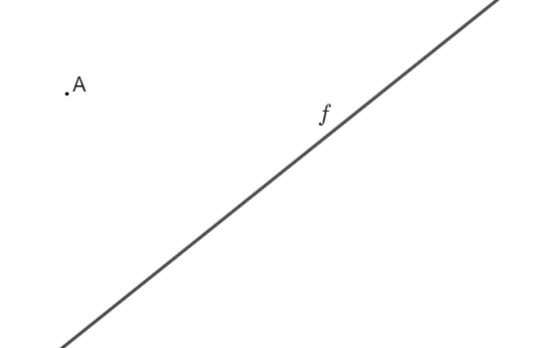
\includegraphics{img/pointAdroiteF.png}
    \end{center}
\end{exercise}

\newpage
\begin{exercise}[points=6]
    Effectue. Laisse tes étapes visibles.
    \begin{enumerate}[cols=3]
        \item $\dfrac{-15}{13} \cdot \dfrac{-39}{45}$
        \item $-\dfrac{-27}{45} - 0,5$
        \item $\left(\dfrac{3}{8} + \dfrac{-7}{2}\right)\cdot \dfrac{15}{12}$
        \item $\dfrac{1}{3}-8+\dfrac{-4}{16}$
        \item $\dfrac{-9}{54} + \dfrac{-72}{8} \cdot \dfrac{-32}{27}$
        \item $1,6 + \dfrac{3}{5} - \left(\dfrac{5}{15}\right)^3$
    \end{enumerate}
\end{exercise}

\begin{exercise}[points=10]
    Effectue les équations suivantes. Laisse ta démarche visible.
    \begin{enumerate}[cols=2, itemsep=0.7cm]
        \item \(3x - 7 = 8\)
        \item \(2x + 7 = 10 - x\)
        \item \(\dfrac{3x}{7} = \dfrac{5}{12}\)
        \item \(\dfrac{1}{2} + \dfrac{6x}{5} = \dfrac{7}{2}\)
        \item \(2(3x + 7) - 13 = 5x + 7 - 5\)
        \item \((3x + 2)^2 - 5x = 10 - 6x + 9x^2\)
        \item \(10 = 2x - 7\)
        \item \(3(5x-1) = 3x\)
        \item \(3x-7 = 7 + 6x\)
        \item \(\dfrac{6}{7} + x = 10\)
    \end{enumerate}
\end{exercise}

\begin{exercise}[points=2]
    \emph{Sur cette feuille} \\
    Trace le cercle tangent à la droite $a$ dont le centre est $A$. Laisse tes constructions visibles et code ton dessin. 
    \begin{center}
        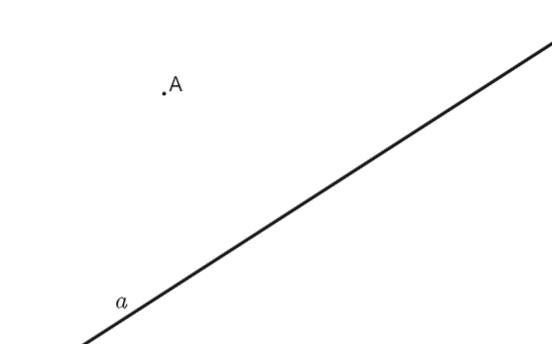
\includegraphics[width=8cm]{img/cercle tangent.png}
    \end{center}
\end{exercise}

\end{document}